\chapter{Diagnóstico de Processos de Degradação Ambiental e Erosão Linear}
\label{cap:degradacao_erosao_linear}

\noindent\tagPratica
\vspace{4pt}

\begin{capObjetivos}
Ao concluir este capítulo, você será capaz de:
\begin{itemize}[leftmargin=1.5em, itemsep=2.5pt]
  \item Explicar a mecânica física e a sequência evolutiva completa da erosão hídrica, do impacto da gota (\textit{splash}) e selamento superficial até sulcos, ravinas e voçorocas (Guerra; Cunha, 1996; Ross, 1994; Cavalcanti, 2006).
  \item Distinguir os mecanismos dominantes em ravinas (escoamento superficial concentrado) e em voçorocas (interseção com o lençol freático, erosão subsuperficial/\textit{piping} e solapamento de taludes).
  \item Diagnosticar processos correlatos em bacias hidrográficas: instabilidade de margens fluviais, degradação de áreas ripárias e assoreamento de canais e reservatórios.
  \item Aplicar a \textbf{Equação Universal de Perda de Solo (USLE)}, $A = R \cdot K \cdot L \cdot S \cdot C \cdot P$, verificando unidades, comparando cenários de manejo e convertendo perdas em massa para taxas de rebaixamento superficial ($\text{mm}\cdot\text{ano}^{-1}$).
  \item Empregar protocolos quantitativos de monitoramento em campo: método dos pinos de erosão, estacas de recuo de cabeceira, perfis transversais de ravinas e fichas padronizadas de avaliação visual.
\end{itemize}
\end{capObjetivos}

\begin{capRevisao}
Este capítulo sintetiza os processos físicos que conectam a qualidade do solo (Capítulo 11) à dinâmica hidrossedimentológica da bacia (Capítulos 7 a 9):
\begin{itemize}[leftmargin=1.5em, itemsep=2.5pt]
  \item \textbf{Infiltração e compactação (Capítulo 11):} quando a intensidade da chuva supera a taxa de infiltração básica ($TIB$), forma-se excedente hídrico superficial (escoamento hortoniano), motor primário da erosão laminar e em sulcos.
  \item \textbf{Conectividade hidrossedimentológica (Capítulo 7):} sedimentos desprendidos nas vertentes só atingem a rede fluvial e assoreiam reservatórios quando existe conectividade topográfica e ausência de faixas ripárias vegetadas.
  \item \textbf{Indicadores PEIR (Capítulo 10):} as taxas medidas pela USLE, por pinos de erosão e por perfis transversais fornecem os indicadores quantitativos de \textbf{Impacto (I)} que justificam o dimensionamento da bioengenharia no Módulo 5.
\end{itemize}
\end{capRevisao}

\etapa{3}{Fundamentação Teórica: Mecânica da Erosão Linear, USLE e Monitoramento}

\begin{boxSimbolo}[Vocabulário Técnico e Símbolos do Capítulo 12]
\begin{itemize}[leftmargin=1.4em, itemsep=2.5pt]
  \item \textbf{\textit{Splash} (salpicamento):} desagregação de partículas do solo pelo impacto cinético direto das gotas de chuva, gerando crosta de selamento superficial.
  \item \textbf{\textit{Piping} (erosão em túneis ou tubular):} remoção interna de partículas finas do solo por fluxos subsuperficiais concentrados, criando dutos que colapsam e aceleram o avanço de voçorocas.
  \item \textbf{USLE ($A = R \cdot K \cdot L \cdot S \cdot C \cdot P$):} modelo empírico que estima a perda média anual de solo por erosão laminar e em sulcos ($\text{t}\cdot\text{ha}^{-1}\cdot\text{ano}^{-1}$).
  \item $T$: limite de tolerância de perda de solo ($\text{t}\cdot\text{ha}^{-1}\cdot\text{ano}^{-1}$), correspondente à taxa máxima de erosão compatível com a renovação pedogenética e manutenção da funcionalidade do perfil.
  \item $h$: taxa de rebaixamento da superfície do solo ($\text{mm}\cdot\text{ano}^{-1}$), vinculada à perda de massa pela densidade do solo ($D_s$).
  \item $\Delta \bar{h}$: variação média de exposição em uma malha de pinos de erosão ($\text{mm}$); valores positivos indicam erosão (rebaixamento) e negativos indicam deposição (soterramento).
  \item $SDR$: Razão de Aporte de Sedimentos (\textit{Sediment Delivery Ratio}, adimensional entre $0$ e $1$), fração do solo erodido nas vertentes que efetivamente alcança o exutório ou reservatório da bacia.
\end{itemize}
\end{boxSimbolo}

\section{Mecânica e Sequência Evolutiva da Erosão Hídrica}

A erosão hídrica acelerada resulta do desequilíbrio entre a \textbf{erosividade} (capacidade da chuva e do escoamento de desprender e transportar partículas) e a \textbf{resistência do sistema solo--vegetação} (cobertura, agregação, rugosidade e infiltração). Conforme sintetizam Guerra e Cunha (1996), Ross (1994) e Cavalcanti (2006), o processo evolui em estágios progressivos de severidade física e de custo exponencial de recuperação (Figura~\ref{fig:evolucao_erosao_linear}).

\begin{figure}[H]
  \centering
  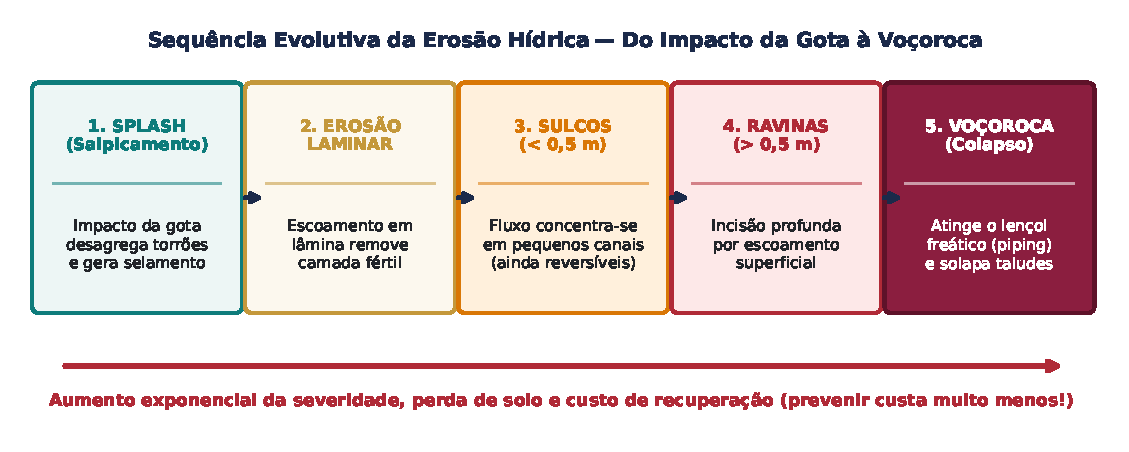
\includegraphics[width=0.94\textwidth]{figures/fig10_evolucao_erosao_linear.pdf}
  \caption{Sequência evolutiva dos processos erosivos hídricos, do impacto da gota (\textit{splash}) ao colapso por voçorocamento, evidenciando o aumento exponencial da severidade e do custo de recuperação.}
  \label{fig:evolucao_erosao_linear}
\end{figure}

Cada estágio possui diagnóstico morfológico e mecânico próprio:
\begin{enumerate}[leftmargin=1.8em, itemsep=3pt]
  \item \textbf{Impacto da gota (\textit{splash}) e selamento superficial:} quando o solo perde cobertura vegetal e serapilheira, as gotas de chuva atingem diretamente os agregados superficiais, rompendo-os e lançando partículas finas (argila e silte) em suspensão. Essas partículas obstruem os poros superficiais, formando uma crosta delgada (\textbf{selamento superficial}) que reduz drasticamente a taxa de infiltração básica.
  \item \textbf{Erosão laminar (entressulcos):} com a infiltração bloqueada pelo selamento ou pela compactação, a água acumula-se e escoa em lâmina difusa sobre a vertente, removendo silenciosamente a camada mais fértil do horizonte A (matéria orgânica, sementes e nutrientes). Por não abrir grandes cicatrizes visíveis no início, costuma passar despercebida até que aflorem raízes, cascalhos ou horizontes subsuperficiais mais claros.
  \item \textbf{Sulcos erosivos ($< 0{,}5\text{ m}$ de profundidade):} irregularidades microtopográficas, marcas de pneus ou linhas de plantio morro abaixo concentram a lâmina d'água em filetes de maior velocidade e tensão cisalhante. Os canais rasos assim abertos são denominados sulcos e, em geral, ainda podem ser corrigidos por práticas conservacionistas e manejo superficial do solo.
  \item \textbf{Ravinas ($> 0{,}5\text{ m}$ de profundidade, sem atingir o lençol freático):} se o escoamento superficial concentrado não for dissipado, os sulcos aprofundam-se e alargam-se, tornando-se incisões permanentes que não são eliminadas por preparo comum do solo. O agente dominante na ravina ainda é o \textbf{escoamento superficial concentrado}, que excava o leito e expande o canal remontantemente (de jusante para montante).
  \item \textbf{Voçorocas (estágio de colapso integrado):} representam a forma mais avançada e destrutiva da erosão linear. Diferenciam-se das ravinas não apenas pelas dimensões métricas, mas sobretudo pelo \textbf{processo hidrogeomorfológico}: a incisão atinge o \textbf{lençol freático} (ou zonas de fluxo subsuperficial saturado). Passam então a atuar simultaneamente o escoamento superficial, a erosão subsuperficial em túneis (\textbf{\textit{piping}}) e a exfiltração na base das paredes, provocando \textbf{solapamento} e escorregamentos sucessivos dos taludes laterais e da cabeceira, mesmo em períodos sem chuva intensa.
\end{enumerate}

\begin{figure}[H]
  \centering
  \begin{minipage}[t]{0.48\textwidth}
    \centering
    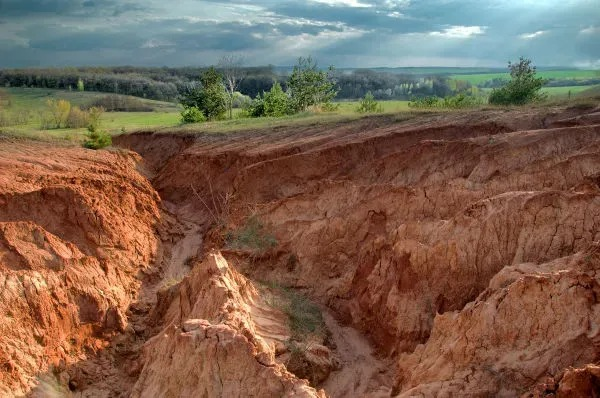
\includegraphics[width=\textwidth,height=4.3cm,keepaspectratio]{figures/foto_vocoroca_severa.jpg}
    \par\small\textbf{(A)} Voçoroca profunda com exposição de horizontes subsuperficiais.
  \end{minipage}\hfill
  \begin{minipage}[t]{0.48\textwidth}
    \centering
    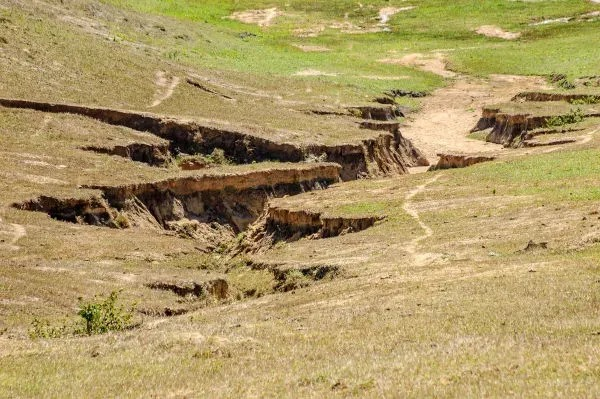
\includegraphics[width=\textwidth,height=4.3cm,keepaspectratio]{figures/foto_pastagem_ravinas.jpg}
    \par\small\textbf{(B)} Cabeceiras erosivas escalonadas em pastagem degradada.
  \end{minipage}
  \caption{\textbf{Registros empíricos de erosão linear severa em vertentes degradadas.} \textit{O que observar:} no painel A, a incisão profunda expõe o perfil pedológico e promove o desmoronamento das paredes laterais por solapamento. No painel B, o avanço regressivo das cabeceiras fragmenta a encosta e intensifica a conectividade de sedimentos para o fundo de vale. Fonte: Acervo didático CHF662.}
  \label{fig:fotos_erosao_linear}
\end{figure}


\section{Instabilidade de Margens Fluviais, Degradação Ripária e Assoreamento}

Na escala da bacia hidrográfica, a erosão das vertentes articula-se diretamente à dinâmica dos canais fluviais e das Áreas de Preservação Permanente (APPs) marginais:
\begin{itemize}[leftmargin=1.5em, itemsep=2.5pt]
  \item \textbf{Degradação ripária e colapso de margens:} a supressão da mata ciliar elimina a malha radicular que confere coesão mecânica aos barrancos (tema aprofundado na bioengenharia do Capítulo 13) e expõe a margem ao impacto direto da corrente fluvial. A erosão na base do talude marginal (\textit{undercutting}) gera quedas em bloco e alargamento desordenado da calha.
  \item \textbf{Assoreamento de canais, açudes e reservatórios:} quando o aporte de sedimentos oriundo das vertentes e margens excede a capacidade de transporte do curso d'água, ocorre deposição no leito. No Semiárido Baiano, o assoreamento reduz rapidamente o volume útil de açudes, barreiros e pequenos barramentos comunitários, agrava a vulnerabilidade hídrica nas estiagens e eleva a turbidez da água.
\end{itemize}

\section{Equação Universal de Perda de Solo (USLE)}

Desenvolvida por Wischmeier e Smith (1978) a partir de milhares de parcelas experimentais e amplamente calibrada para condições tropicais e brasileiras, a \textbf{Equação Universal de Perda de Solo (USLE)} estima a perda média anual de solo por erosão laminar e em sulcos a partir do produto de seis fatores físicos e de manejo.

\begin{boxFormula}[Equação Universal de Perda de Solo (USLE) e Conversão para Rebaixamento]
\[
A = R \cdot K \cdot L \cdot S \cdot C \cdot P
\]
\begin{itemize}[leftmargin=1.4em, itemsep=2pt]
  \item $A$: perda média anual estimada de solo ($\text{t}\cdot\text{ha}^{-1}\cdot\text{ano}^{-1}$).
  \item $R$: fator de \textbf{erosividade da chuva} ($\text{MJ}\cdot\text{mm}\cdot\text{ha}^{-1}\cdot\text{h}^{-1}\cdot\text{ano}^{-1}$); expressa a energia cinética e intensidade máxima das precipitações ao longo do ano.
  \item $K$: fator de \textbf{erodibilidade do solo} ($\text{t}\cdot\text{ha}\cdot\text{h}\cdot\text{ha}^{-1}\cdot\text{MJ}^{-1}\cdot\text{mm}^{-1}$); reflete a suscetibilidade intrínseca do solo à erosão (textura, matéria orgânica, estrutura e permeabilidade).
  \item $L$ e $S$: fatores topográficos de \textbf{comprimento de rampa ($L$)} e \textbf{declividade ($S$)} (adimensionais, frequentemente agrupados como fator $LS$). Quanto maior e mais íngreme a vertente, maior o valor de $LS$.
  \item $C$: fator de \textbf{uso, manejo e cobertura vegetal} (adimensional, entre $\approx 0{,}001$ em floresta densa e $1{,}00$ em solo continuamente descoberto e mobilizado).
  \item $P$: fator de \textbf{práticas conservacionistas} (adimensional, de $1{,}00$ em plantio morro abaixo até $\approx 0{,}50$ em plantio em contorno ou $0{,}20$--$0{,}40$ com terraceamento e cordões vegetados).
\end{itemize}

\textbf{Relação entre Perda de Massa ($A$) e Rebaixamento Superficial ($h$):}
Como $1\text{ ha} = 10.000\text{ m}^2$, uma lâmina de $1\text{ mm}$ ($0{,}001\text{ m}$) de solo em $1\text{ ha}$ possui volume de $10\text{ m}^3$. Multiplicando pela densidade do solo ($D_s$ em $\text{t}\cdot\text{m}^{-3} = \text{g}\cdot\text{cm}^{-3}$), cada $1\text{ mm}$ corresponde a $10 \cdot D_s$ toneladas por hectare:
\[
h\,(\text{mm}\cdot\text{ano}^{-1}) = \frac{A\,(\text{t}\cdot\text{ha}^{-1}\cdot\text{ano}^{-1})}{10 \cdot D_s} \qquad \Longleftrightarrow \qquad A = 10 \cdot D_s \cdot h
\]
\end{boxFormula}

É fundamental destacar duas características essenciais da USLE: (1) o produto $R \cdot K \cdot L \cdot S$ representa o \textbf{potencial natural de erosão} (o solo completamente descoberto e sem práticas conservacionistas); e (2) os fatores $C$ e $P$ são os elementos sobre os quais a gestão territorial e o manejo atuam diretamente, podendo reduzir as perdas em mais de $95\%$, conforme ilustrado na Figura~\ref{fig:usle_sensibilidade}. Além disso, a USLE \textbf{não modela erosão em ravinas profundas, voçorocas ou margens fluviais}, nem quantifica diretamente a deposição na base da vertente. Para estimar o sedimento que chega a um reservatório, associa-se a USLE à Razão de Aporte de Sedimentos ($SDR$).

\begin{figure}[H]
  \centering
  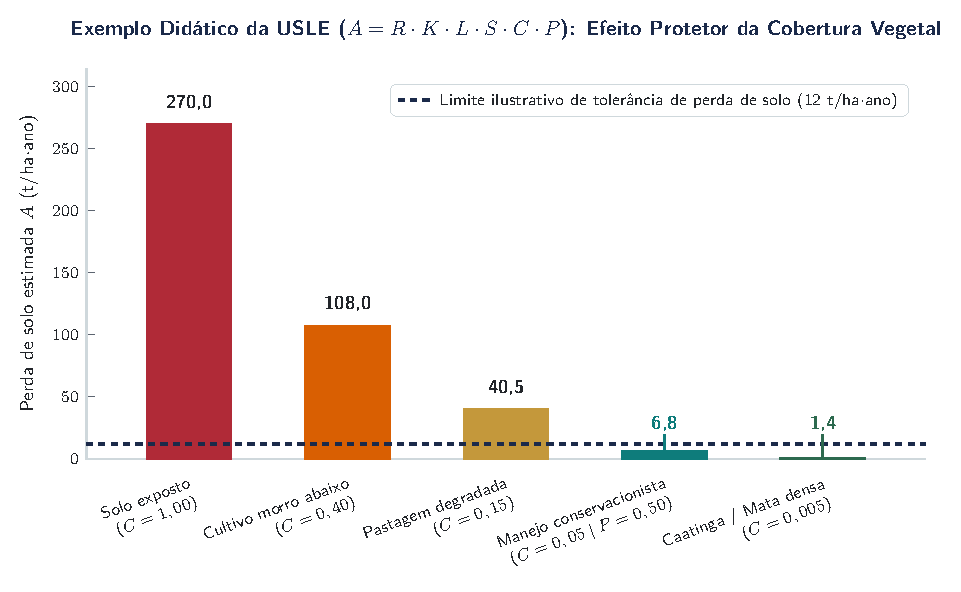
\includegraphics[width=0.88\textwidth]{figures/fig11_usle_sensibilidade.pdf}
  \caption{Análise de sensibilidade da Equação Universal de Perda de Solo ($R = 6.000$, $K = 0{,}03$, $LS = 1{,}5$, potencial natural de $270\text{ t}\cdot\text{ha}^{-1}\cdot\text{ano}^{-1}$) sob cinco cenários de cobertura e manejo frente ao limite ilustrativo de tolerância ($12\text{ t}\cdot\text{ha}^{-1}\cdot\text{ano}^{-1}$).}
  \label{fig:usle_sensibilidade}
\end{figure}

\section{Protocolos Quantitativos de Diagnóstico e Monitoramento em Campo}

Modelos como a USLE fornecem estimativas de planejamento, mas o diagnóstico rigoroso de processos ativos em campo requer medições diretas e rastreáveis:
\begin{enumerate}[leftmargin=1.8em, itemsep=2.5pt]
  \item \textbf{Método dos Pinos de Erosão:} consiste na cravação vertical de vergalhões metálicos ou pinos rígidos (tipicamente de $30$ a $50\text{ cm}$ de comprimento) dispostos em malha ou transectos ao longo da vertente ou talude, deixando uma altura inicial exposta padronizada (ex.: $150\text{ mm}$) marcada com anilha ou pintura. Após cada evento chuvoso ou ciclo anual, mede-se novamente a altura exposta com paquímetro ou régua milimetrada: aumento na altura exposta ($\Delta h > 0$) registra \textbf{rebaixamento erosivo}; diminuição ($\Delta h < 0$) indica \textbf{deposição local de sedimentos}.
  \item \textbf{Estacas de Monitoramento de Recuo de Cabeceira e Bordas:} em ravinas e voçorocas ativas, instalam-se estacas fixas externas a distâncias conhecidas (ex.: $2{,}0$ a $5{,}0\text{ m}$ além da borda instável) em alinhamentos radiais. Medições periódicas da distância entre cada estaca e a borda do talude permitem calcular a taxa de avanço remontante ($\text{m}\cdot\text{ano}^{-1}$).
  \item \textbf{Perfis Transversais de Ravinas e Voçorocas:} em seções fixas espaçadas regularmente pela distância $L_{\text{seg}}$ ao longo do canal erosivo, mede-se a largura superior ($B$), a largura de fundo ($b$) e a profundidade vertical média ($h_{\text{rav}}$) a partir de uma linha de referência nivelada (trena esticada entre estacas), estimando a área da seção trapezoidal por $A = \frac{B + b}{2}\cdot h_{\text{rav}}$. Integrando as áreas transversais ($A_1, A_2, \dots$) pelo método da média das áreas, obtém-se o volume de solo mobilizado ($V = \frac{A_1 + A_2}{2}\cdot L_{\text{seg}}$) e sua massa ($M = V \cdot D_s$).
  \item \textbf{Fichas Padronizadas de Avaliação Visual:} complementam as medições métricas registrando coordenadas geográficas, posição na vertente, cobertura vegetal estimada, presença de selamento, exfiltração subsuperficial (surgências na parede da voçoroca), conectividade com cursos d'água e registro fotográfico com escala métrica.
\end{enumerate}

\etapa{4}{Estudos de Caso e Exemplos Resolvidos Passo a Passo}

\begin{boxExemplo}{12.1 (Básico)}{Aplicação da USLE e Comparação de Cenários de Manejo (Figura~\ref{fig:usle_sensibilidade})}
\passoEnunciado{Uma vertente no Semiárido Baiano apresenta os seguintes fatores físicos naturais: erosividade da chuva $R = 6.000\text{ MJ}\cdot\text{mm}\cdot\text{ha}^{-1}\cdot\text{h}^{-1}\cdot\text{ano}^{-1}$, erodibilidade do solo $K = 0{,}03\text{ t}\cdot\text{ha}\cdot\text{h}\cdot\text{ha}^{-1}\cdot\text{MJ}^{-1}\cdot\text{mm}^{-1}$ e fator topográfico combinado $LS = 1{,}5$. O limite ilustrativo de tolerância de perda de solo adotado para o local é $T = 12{,}0\text{ t}\cdot\text{ha}^{-1}\cdot\text{ano}^{-1}$.}
\passoDados{Cinco cenários de uso e manejo: (1) solo exposto ($C = 1{,}00$; $P = 1{,}00$); (2) cultivo morro abaixo ($C = 0{,}40$; $P = 1{,}00$); (3) pastagem degradada ($C = 0{,}15$; $P = 1{,}00$); (4) manejo conservacionista em contorno ($C = 0{,}05$; $P = 0{,}50$); e (5) Caatinga densa preservada ($C = 0{,}005$; $P = 1{,}00$).}
\passoPedido{Calcular a perda anual estimada ($A$) em cada cenário, verificar quais atendem ao limite de tolerância ($A \le 12{,}0$) e calcular a redução percentual promovida pelo manejo conservacionista em relação ao cultivo morro abaixo.}
\passoMetodo{Cálculo prévio do potencial natural de erosão ($PNE = R \cdot K \cdot LS$) seguido da multiplicação pelos fatores $C$ e $P$ de cada cenário.}
\passoContas{
\textbf{Etapa 1, Potencial Natural de Erosão ($PNE$):}
\[
PNE = R \cdot K \cdot LS = 6.000 \times 0{,}03 \times 1{,}5 = 180 \times 1{,}5 = 270{,}0\text{ t}\cdot\text{ha}^{-1}\cdot\text{ano}^{-1}
\]
Note que as unidades de $\text{MJ}$, $\text{mm}$, $\text{h}$ e um fator $\text{ha}$ cancelam-se rigorosamente entre $R$ e $K$, restando $\text{t}\cdot\text{ha}^{-1}\cdot\text{ano}^{-1}$.

\textbf{Etapa 2, Perda de solo ($A$) nos cinco cenários:}
\begin{align*}
  A_1\; (\text{solo exposto}) &= 270{,}0 \times 1{,}00 \times 1{,}00 = 270{,}0\text{ t}\cdot\text{ha}^{-1}\cdot\text{ano}^{-1} \quad (> 12\text{, crítico}) \\
  A_2\; (\text{cultivo morro abaixo}) &= 270{,}0 \times 0{,}40 \times 1{,}00 = 108{,}0\text{ t}\cdot\text{ha}^{-1}\cdot\text{ano}^{-1} \quad (> 12\text{, insustentável}) \\
  A_3\; (\text{pastagem degradada}) &= 270{,}0 \times 0{,}15 \times 1{,}00 = 40{,}5\text{ t}\cdot\text{ha}^{-1}\cdot\text{ano}^{-1} \quad (> 12\text{, acima do limite}) \\
  A_4\; (\text{manejo conservacionista}) &= 270{,}0 \times 0{,}05 \times 0{,}50 = 6{,}75\text{ t}\cdot\text{ha}^{-1}\cdot\text{ano}^{-1} \quad (\le 12\text{, sustentável}) \\
  A_5\; (\text{Caatinga densa}) &= 270{,}0 \times 0{,}005 \times 1{,}00 = 1{,}35\text{ t}\cdot\text{ha}^{-1}\cdot\text{ano}^{-1} \quad (\le 12\text{, referência})
\end{align*}
\textbf{Etapa 3, Redução do manejo conservacionista ($A_4$) frente ao cultivo morro abaixo ($A_2$):}
\[
\text{Redução} = \frac{108{,}0 - 6{,}75}{108{,}0}\times 100\% = \frac{101{,}25}{108{,}0}\times 100\% = 93{,}75\%
\]}
\passoResposta{Perdas: $270{,}0$ (solo exposto), $108{,}0$ (morro abaixo), $40{,}5$ (pastagem degradada), $6{,}75$ (manejo conservacionista) e $1{,}35\text{ t}\cdot\text{ha}^{-1}\cdot\text{ano}^{-1}$ (Caatinga). Apenas os cenários 4 e 5 atendem ao limite $T = 12\text{ t}\cdot\text{ha}^{-1}\cdot\text{ano}^{-1}$; o manejo conservacionista reduz a erosão em $93{,}75\%$.}
\passoVerificacao{Os valores coincidem integralmente com as barras da Figura~\ref{fig:usle_sensibilidade} (onde $6{,}75$ e $1{,}35$ aparecem arredondados para uma casa decimal: $6{,}8$ e $1{,}4$) e demonstram que a cobertura do solo ($C$) exerce impacto decisivo no controle da erosão.}
\end{boxExemplo}

\begin{boxExemplo}{12.2 (Intermediário)}{Conversão de Perda de Solo (USLE) em Espessura de Rebaixamento Superficial}
\passoEnunciado{Para comunicar a agricultores e gestores o significado físico da perda de solo obtida no cenário de cultivo morro abaixo do Exemplo~12.1 ($A = 108{,}0\text{ t}\cdot\text{ha}^{-1}\cdot\text{ano}^{-1}$), converta essa taxa em espessura anual de solo removido e estime quanto do horizonte A será perdido em $25$ anos.}
\passoDados{$A = 108{,}0\text{ t}\cdot\text{ha}^{-1}\cdot\text{ano}^{-1}$; densidade do solo da camada superficial $D_s = 1{,}35\text{ g}\cdot\text{cm}^{-3} = 1{,}35\text{ t}\cdot\text{m}^{-3}$; horizonte temporal de análise $= 25\text{ anos}$.}
\passoPedido{Calcular a taxa anual de rebaixamento $h$ ($\text{mm}\cdot\text{ano}^{-1}$) e a espessura acumulada removida em $25$ anos (em $\text{cm}$).}
\passoMetodo{Aplicação da relação geométrica $h = A / (10 \cdot D_s)$ e multiplicação pelo horizonte de $25$ anos.}
\passoContas{
\textbf{Etapa 1, Massa correspondente a $1\text{ mm}$ de solo em $1\text{ ha}$:}
\[
M_{1\text{mm}} = 10 \cdot D_s = 10 \times 1{,}35 = 13{,}5\text{ t}\cdot\text{ha}^{-1}\cdot\text{mm}^{-1}
\]
\textbf{Etapa 2, Rebaixamento anual:}
\[
h = \frac{108{,}0}{13{,}5} = 8{,}00\text{ mm}\cdot\text{ano}^{-1}
\]
\textbf{Etapa 3, Rebaixamento acumulado em $25$ anos:}
\[
H_{25} = 8{,}00\text{ mm}\cdot\text{ano}^{-1} \times 25\text{ anos} = 200{,}0\text{ mm} = 20{,}0\text{ cm}
\]}
\passoResposta{Taxa de rebaixamento de $8{,}00\text{ mm}\cdot\text{ano}^{-1}$, removendo $20{,}0\text{ cm}$ de solo superficial em apenas $25$ anos.}
\passoVerificacao{Em solos rasos do Semiárido Baiano (como Neossolos Litólicos e Luvissolos com horizonte A entre $15$ e $25\text{ cm}$), perder $20\text{ cm}$ em um quarto de século significa eliminar completamente a camada biologicamente ativa e expor o horizonte B ou a rocha alterada, processo clássico de desertificação edáfica.}
\end{boxExemplo}

\begin{boxExemplo}{12.3 (Intermediário)}{Monitoramento de Talude pelo Método dos Pinos de Erosão}
\passoEnunciado{Cinco pinos de erosão foram instalados ao longo de um perfil de talude exposto próximo à estrada de acesso de um empreendimento, todos com altura inicial exposta padronizada de $150\text{ mm}$. Após um ciclo hidrológico de $12$ meses, novas leituras foram coletadas com paquímetro.}
\passoDados{Altura inicial exposta em todos os pinos: $h_0 = 150\text{ mm}$. Leituras após $12$ meses (do topo à base do talude): Pino 1 $= 168\text{ mm}$; Pino 2 $= 174\text{ mm}$; Pino 3 $= 162\text{ mm}$; Pino 4 $= 156\text{ mm}$; Pino 5 (sopé do talude) $= 140\text{ mm}$. Densidade do solo local: $D_s = 1{,}40\text{ g}\cdot\text{cm}^{-3}$.}
\passoPedido{Calcular a variação $\Delta h_i$ em cada pino, o balanço líquido médio de rebaixamento ($\Delta \bar{h}$) e a perda líquida equivalente de solo em $\text{t}\cdot\text{ha}^{-1}\cdot\text{ano}^{-1}$.}
\passoMetodo{Cálculo individual $\Delta h_i = h_{1,i} - h_0$ (respeitando sinais positivos para erosão e negativos para deposição), média aritmética e conversão via $A = 10 \cdot D_s \cdot \Delta \bar{h}$.}
\passoContas{
\textbf{Etapa 1, Variação em cada pino:}
\begin{align*}
  \Delta h_1 &= 168 - 150 = +18\text{ mm} \quad (\text{erosão}) \\
  \Delta h_2 &= 174 - 150 = +24\text{ mm} \quad (\text{erosão máxima no terço médio}) \\
  \Delta h_3 &= 162 - 150 = +12\text{ mm} \quad (\text{erosão}) \\
  \Delta h_4 &= 156 - 150 = +6\text{ mm} \quad (\text{erosão moderada}) \\
  \Delta h_5 &= 140 - 150 = -10\text{ mm} \quad (\text{deposição no sopé})
\end{align*}
\textbf{Etapa 2, Balanço líquido médio ($\Delta \bar{h}$):}
\[
\Delta \bar{h} = \frac{18 + 24 + 12 + 6 + (-10)}{5} = \frac{50}{5} = +10{,}0\text{ mm}\cdot\text{ano}^{-1}
\]
\textbf{Etapa 3, Perda líquida equivalente de solo:}
\[
A_{\text{pinos}} = 10 \times 1{,}40 \times 10{,}0 = 140{,}0\text{ t}\cdot\text{ha}^{-1}\cdot\text{ano}^{-1}
\]}
\passoResposta{Rebaixamento líquido médio de $10{,}0\text{ mm}\cdot\text{ano}^{-1}$, correspondente a uma perda líquida equivalente de $140{,}0\text{ t}\cdot\text{ha}^{-1}\cdot\text{ano}^{-1}$.}
\passoVerificacao{O sinal negativo no Pino 5 ($-10\text{ mm}$) é fisicamente esperado em encostas: parte do sedimento removido dos segmentos superiores e médios deposita-se no sopé com a redução da declividade. Desconsiderar o sinal negativo superestimaria o balanço líquido da encosta.}
\end{boxExemplo}

\begin{boxExemplo}{12.4 (Avançado)}{Cubagem de Solo Mobilizado em Ravina por Perfis Transversais}
\passoEnunciado{Para dimensionar estruturas de contenção em uma ravina ativa com $40{,}0\text{ m}$ de extensão, uma equipe levantou duas seções transversais representativas (Seção 1 a montante e Seção 2 a jusante), ambas aproximadas por geometria trapezoidal.}
\passoDados{Comprimento do trecho entre seções: $L = 40{,}0\text{ m}$. Seção 1: largura de topo $B_1 = 3{,}2\text{ m}$, largura de fundo $b_1 = 1{,}2\text{ m}$, profundidade $h_1 = 1{,}5\text{ m}$. Seção 2: $B_2 = 4{,}0\text{ m}$, $b_2 = 1{,}6\text{ m}$, profundidade $h_2 = 2{,}0\text{ m}$. Densidade média do solo do perfil: $D_s = 1{,}45\text{ t}\cdot\text{m}^{-3}$.}
\passoPedido{Calcular a área de cada seção ($A_1$ e $A_2$), o volume total de solo escavado ($V$) pelo método da média das áreas e a massa total mobilizada ($M$).}
\passoMetodo{Área do trapézio $A = \frac{B + b}{2}\cdot h$, volume prismoidal simplificado $V = \frac{A_1 + A_2}{2}\cdot L$ e conversão para massa $M = V \cdot D_s$.}
\passoContas{
\textbf{Etapa 1, Área das seções transversais:}
\[
A_1 = \frac{3{,}2 + 1{,}2}{2}\times 1{,}5 = \frac{4{,}4}{2}\times 1{,}5 = 2{,}2 \times 1{,}5 = 3{,}30\text{ m}^2
\]
\[
A_2 = \frac{4{,}0 + 1{,}6}{2}\times 2{,}0 = \frac{5{,}6}{2}\times 2{,}0 = 2{,}8 \times 2{,}0 = 5{,}60\text{ m}^2
\]
\textbf{Etapa 2, Volume total mobilizado no trecho de $40\text{ m}$:}
\[
V = \frac{3{,}30 + 5{,}60}{2}\times 40{,}0 = \frac{8{,}90}{2}\times 40{,}0 = 4{,}45 \times 40{,}0 = 178{,}0\text{ m}^3
\]
\textbf{Etapa 3, Massa total de solo mobilizada:}
\[
M = 178{,}0\text{ m}^3 \times 1{,}45\text{ t}\cdot\text{m}^{-3} = 258{,}1\text{ t}
\]}
\passoResposta{$A_1 = 3{,}30\text{ m}^2$, $A_2 = 5{,}60\text{ m}^2$, volume escavado $V = 178{,}0\text{ m}^3$ e massa mobilizada de $258{,}1\text{ toneladas}$ de solo.}
\passoVerificacao{Para visualizar a magnitude do impacto, $178\text{ m}^3$ equivalem a aproximadamente $15$ a $18$ caminhões basculantes convencionais carregados de solo removidos de uma única ravina de $40\text{ m}$, grande parte dos quais segue diretamente para drenagens e açudes a jusante.}
\end{boxExemplo}

\begin{boxExemplo}{12.5 (Avançado)}{Estimativa de Assoreamento de Reservatório por USLE e Razão de Aporte ($SDR$)}
\passoEnunciado{Uma microbacia rural de $250\text{ ha}$ no Semiárido Baiano drena para um açude comunitário com capacidade inicial de armazenamento de $160.000\text{ m}^3$. Estudos anteriores estimaram perda média de solo pela USLE de $A = 32{,}0\text{ t}\cdot\text{ha}^{-1}\cdot\text{ano}^{-1}$ na microbacia e Razão de Aporte de Sedimentos $SDR = 0{,}25$ (isto é, $25\%$ do solo erodido nas vertentes atinge o reservatório).}
\passoDados{Área da microbacia: $250\text{ ha}$; perda média USLE: $A = 32{,}0\text{ t}\cdot\text{ha}^{-1}\cdot\text{ano}^{-1}$; $SDR = 0{,}25$; densidade aparente do sedimento depositado no fundo do açude: $\rho_{\text{sed}} = 1{,}25\text{ t}\cdot\text{m}^{-3}$; capacidade útil inicial: $V_0 = 160.000\text{ m}^3$.}
\passoPedido{Calcular (a) a produção anual de sedimentos que chega ao açude ($Y$, em $\text{t}\cdot\text{ano}^{-1}$); (b) o volume assoreado por ano ($V_{\text{sed}}$); e (c) o percentual da capacidade inicial perdido em $20$ anos caso não haja conservação na microbacia.}
\passoMetodo{Cálculo do aporte de sedimentos $Y = A \cdot \text{Área} \cdot SDR$, conversão para volume ($V_{\text{sed}} = Y / \rho_{\text{sed}}$) e projeção linear de $20$ anos frente ao volume inicial.}
\passoContas{
\textbf{Etapa 1, Aporte anual de sedimentos no reservatório ($Y$):}
\[
Y = 32{,}0\text{ t}\cdot\text{ha}^{-1}\cdot\text{ano}^{-1} \times 250\text{ ha} \times 0{,}25 = 8.000 \times 0{,}25 = 2.000{,}0\text{ t}\cdot\text{ano}^{-1}
\]
\textbf{Etapa 2, Volume anual de assoreamento ($V_{\text{sed}}$):}
\[
V_{\text{sed}} = \frac{2.000{,}0\text{ t}\cdot\text{ano}^{-1}}{1{,}25\text{ t}\cdot\text{m}^{-3}} = 1.600{,}0\text{ m}^3\cdot\text{ano}^{-1}
\]
\textbf{Etapa 3, Volume assoreado em $20$ anos e perda percentual de capacidade:}
\[
V_{20} = 1.600{,}0 \times 20 = 32.000{,}0\text{ m}^3
\]
\[
\text{Perda percentual} = \frac{32.000{,}0}{160.000{,}0}\times 100\% = 20{,}0\%
\]}
\passoResposta{Aporte anual de $2.000{,}0\text{ t}\cdot\text{ano}^{-1}$ ($1.600{,}0\text{ m}^3\cdot\text{ano}^{-1}$), provocando perda de $20{,}0\%$ da capacidade de armazenamento do açude em $20$ anos.}
\passoVerificacao{O resultado demonstra a conexão indissociável entre manejo de solos nas vertentes e segurança hídrica no Semiárido: sem controle erosivo na microbacia (redução de $C$ e $P$ e recomposição ripária), um quinto do volume do reservatório desaparece em duas décadas.}
\end{boxExemplo}

\etapa{5}{Erros Mais Comuns e Como Evitá-los}

\begin{boxErro}[Erro 1: Chamar Qualquer Canal Erosivo Profundo de Voçoroca]
\textbf{Equívoco frequente:} Classificar qualquer incisão com mais de $1\text{ m}$ de profundidade automaticamente como voçoroca sem investigar a presença de água subsuperficial.\par
\textbf{Correção técnica:} A distinção geomorfológica entre \textbf{ravina} e \textbf{voçoroca} baseia-se no mecanismo dominante: ravinas são escavadas exclusivamente por escoamento superficial concentrado; voçorocas interceptam o lençol freático ou fluxos subsuperficiais concentrados, apresentando \textit{piping}, surgências de água e solapamento de taludes. Esse diagnóstico muda radicalmente o projeto de recuperação (voçorocas exigem drenagem subsuperficial além do desvio de águas superficiais).
\end{boxErro}

\begin{boxErro}[Erro 2: Aplicar a USLE para Estimar Erosão em Voçorocas ou Margens Fluviais]
\textbf{Equívoco frequente:} Usar $A = R \cdot K \cdot L \cdot S \cdot C \cdot P$ como se o resultado englobasse toda a produção de sedimentos de uma bacia com voçorocas ativas e desmoronamento de margens.\par
\textbf{Correção técnica:} A USLE foi calibrada exclusivamente para \textbf{erosão laminar e em sulcos} nas vertentes. Processos lineares profundos (ravinas e voçorocas) e erosão marginal devem ser quantificados separadamente por perfis transversais, estacas de recuo, levantamento topográfico ou fotogrametria com drone.
\end{boxErro}

\begin{boxErro}[Erro 3: Misturar Unidades Métricas e Inglesas nos Fatores $R$ e $K$ da USLE]
\textbf{Equívoco frequente:} Multiplicar um fator $R$ no Sistema Internacional ($\text{MJ}\cdot\text{mm}\cdot\text{ha}^{-1}\cdot\text{h}^{-1}\cdot\text{ano}^{-1}$) por um fator $K$ retirado de tabelas antigas em unidades norte-americanas sem conversão.\par
\textbf{Correção técnica:} Confira sempre a análise dimensional de $R \cdot K$: no Sistema Internacional, o produto $R \cdot K$ deve resultar diretamente em $\text{t}\cdot\text{ha}^{-1}\cdot\text{ano}^{-1}$. Divergências de ordem de grandeza ($10\times$ ou $100\times$) quase sempre denunciam incompatibilidade de unidades entre $R$ e $K$.
\end{boxErro}

\begin{boxErro}[Erro 4: Ignorar Pinos com Valores Negativos (Deposição) no Balanço de Vertente]
\textbf{Equívoco frequente:} Descartar ou tomar em módulo as leituras de pinos parcialmente soterrados na base de uma encosta.\par
\textbf{Correção técnica:} Pinos com $\Delta h < 0$ registram redistribuição interna de sedimentos (deposição). Para estimar o balanço líquido da vertente, preserva-se o sinal algébrico na média; para analisar separadamente a zona de perda máxima, reportam-se ambos os valores (erosão bruta nos segmentos de perda e balanço líquido total).
\end{boxErro}

\etapa{6}{Exercícios de Fixação}

\subsection*{Nível Básico (Processos Erosivos, Morfologia e Conceitos)}

\begin{enumerate}[leftmargin=1.8em, itemsep=6pt]
  \item Descreva o papel do \textbf{impacto da gota de chuva (\textit{splash})} na formação do selamento superficial e explique como esse fenômeno acelera o surgimento da erosão laminar.
  \espacoResolucao[1.8cm]

  \item Estabeleça a diferença técnica entre \textbf{sulco}, \textbf{ravina} e \textbf{voçoroca} quanto aos processos hidrológicos atuantes e à reversibilidade por manejo convencional.
  \espacoResolucao[1.8cm]

  \item O que é \textbf{\textit{piping}} e por que sua identificação em campo é decisiva antes de propor obras de estabilização em uma encosta?
  \espacoResolucao[1.8cm]

  \item Explique o significado físico de cada um dos seis fatores da Equação Universal de Perda de Solo ($A = R \cdot K \cdot L \cdot S \cdot C \cdot P$) e indique quais dois fatores podem ser diretamente modificados pelo manejo conservacionista.
  \espacoResolucao[1.8cm]

  \item Explique como a degradação de áreas ripárias (matas ciliares) contribui simultaneamente para a instabilidade de margens fluviais e para o assoreamento de reservatórios.
  \espacoResolucao[1.8cm]
\end{enumerate}

\subsection*{Nível Intermediário (Cálculos de USLE, Pinos, Perfis e Assoreamento)}

\begin{enumerate}[leftmargin=1.8em, itemsep=6pt, resume]
  \item Uma área agrícola apresenta $R = 5.000\text{ MJ}\cdot\text{mm}\cdot\text{ha}^{-1}\cdot\text{h}^{-1}\cdot\text{ano}^{-1}$, $K = 0{,}025\text{ t}\cdot\text{ha}\cdot\text{h}\cdot\text{ha}^{-1}\cdot\text{MJ}^{-1}\cdot\text{mm}^{-1}$, $LS = 2{,}0$ e fator de manejo $C = 0{,}20$. Calcule a perda anual de solo ($A$) sob plantio morro abaixo ($P = 1{,}00$) e sob plantio em contorno ($P = 0{,}50$).
  \espacoResolucao[2.2cm]

  \item Uma vertente submetida a uso intensivo registra perda anual estimada de $A = 70{,}0\text{ t}\cdot\text{ha}^{-1}\cdot\text{ano}^{-1}$ em um solo com densidade $D_s = 1{,}40\text{ g}\cdot\text{cm}^{-3}$. Calcule o rebaixamento anual da superfície ($h$, em $\text{mm}\cdot\text{ano}^{-1}$) e a espessura acumulada perdida em $20$ anos (em $\text{cm}$).
  \espacoResolucao[2.2cm]

  \item Quatro pinos de erosão instalados em uma encosta registraram, após um ano, as seguintes variações de altura exposta ($\Delta h$): $+14\text{ mm}$, $+18\text{ mm}$, $+10\text{ mm}$ e $-2\text{ mm}$. Sabendo que a densidade do solo é $D_s = 1{,}30\text{ g}\cdot\text{cm}^{-3}$, calcule o rebaixamento líquido médio ($\Delta \bar{h}$) e a perda líquida equivalente em $\text{t}\cdot\text{ha}^{-1}\cdot\text{ano}^{-1}$.
  \espacoResolucao[2.2cm]

  \item Uma ravina com $30{,}0\text{ m}$ de extensão teve duas seções transversais trapezoidais medidas: Seção 1 ($B_1 = 2{,}4\text{ m}$; $b_1 = 0{,}8\text{ m}$; $h_1 = 1{,}0\text{ m}$) e Seção 2 ($B_2 = 3{,}6\text{ m}$; $b_2 = 1{,}2\text{ m}$; $h_2 = 1{,}5\text{ m}$). Considerando $D_s = 1{,}50\text{ t}\cdot\text{m}^{-3}$, calcule o volume total ($V$) e a massa ($M$) de solo mobilizado.
  \espacoResolucao[2.2cm]

  \item Uma microbacia de $400\text{ ha}$ apresenta perda média de solo $A = 25{,}0\text{ t}\cdot\text{ha}^{-1}\cdot\text{ano}^{-1}$ e $SDR = 0{,}20$, drenando para um açude de $80.000\text{ m}^3$ de capacidade útil inicial. Adotando $\rho_{\text{sed}} = 1{,}25\text{ t}\cdot\text{m}^{-3}$, calcule o volume anual assoreado e o percentual de capacidade perdido em $10$ anos.
  \espacoResolucao[2.2cm]
\end{enumerate}

\subsection*{Nível Aplicado (Questões Objetivas A--E)}

\begin{enumerate}[leftmargin=1.8em, itemsep=6pt, resume]
  \item Na sequência evolutiva da erosão hídrica (Guerra; Cunha, 1996), a transição de uma ravina para uma voçoroca caracteriza-se fundamentalmente por:
  \begin{alternativas}
    \item Interrupção completa do escoamento superficial durante os eventos de chuva.
    \item Interseção da incisão com o lençol freático ou fluxos subsuperficiais concentrados, desencadeando \textit{piping} e solapamento de taludes.
    \item Reversibilidade imediata por uma única operação de aração rasa do solo.
    \item Deposição contínua de matéria orgânica que fecha naturalmente o canal em poucos meses.
    \item Ausência de recuo remontante na cabeceira da feição erosiva.
  \end{alternativas}

  \item A respeito das limitações metodológicas da Equação Universal de Perda de Solo (USLE), assinale a alternativa correta:
  \begin{alternativas}
    \item A USLE quantifica diretamente o volume escavado em grandes voçorocas causadas por \textit{piping}.
    \item O fator $K$ representa a energia cinética das chuvas e depende exclusivamente do regime climático regional.
    \item A USLE estima a perda média anual por erosão laminar e em sulcos nas vertentes, não computando diretamente erosão em voçorocas, margens fluviais nem deposição ao longo do trajeto sem o uso do $SDR$.
    \item A redução do fator $C$ por meio de cobertura vegetal aumenta proporcionalmente a perda de solo $A$.
    \item O produto $C \cdot P$ representa o potencial natural de erosão de uma bacia independente da ação humana.
  \end{alternativas}

  \item Uma parcela experimental apresenta $R = 4.000\text{ MJ}\cdot\text{mm}\cdot\text{ha}^{-1}\cdot\text{h}^{-1}\cdot\text{ano}^{-1}$, $K = 0{,}04\text{ t}\cdot\text{ha}\cdot\text{h}\cdot\text{ha}^{-1}\cdot\text{MJ}^{-1}\cdot\text{mm}^{-1}$, $LS = 1{,}5$, $C = 0{,}10$ e $P = 0{,}50$. A perda média anual de solo ($A$) estimada pela USLE é:
  \begin{alternativas}
    \item $6{,}0\text{ t}\cdot\text{ha}^{-1}\cdot\text{ano}^{-1}$.
    \item $12{,}0\text{ t}\cdot\text{ha}^{-1}\cdot\text{ano}^{-1}$.
    \item $24{,}0\text{ t}\cdot\text{ha}^{-1}\cdot\text{ano}^{-1}$.
    \item $48{,}0\text{ t}\cdot\text{ha}^{-1}\cdot\text{ano}^{-1}$.
    \item $240{,}0\text{ t}\cdot\text{ha}^{-1}\cdot\text{ano}^{-1}$.
  \end{alternativas}

  \item No monitoramento de processos erosivos em campo, o método mais adequado para mensurar a taxa anual de recuo remontante da cabeceira de uma voçoroca ativa é:
  \begin{alternativas}
    \item Determinação de pH e saturação por bases em laboratório.
    \item Instalação de estacas fixas de referência externas à borda instável com medições periódicas de distância até a escarpa.
    \item Uso isolado de infiltrômetro de anel dentro do leito alagado do rio principal.
    \item Cálculo exclusivo do fator $R$ a partir da precipitação média mensal.
    \item Estimativa visual sem marco fixo nem registro de data.
  \end{alternativas}

  \item Em uma parcela monitorada com quatro pinos de erosão durante $12$ meses, as variações de altura exposta foram $+12\text{ mm}$, $+8\text{ mm}$, $+16\text{ mm}$ e $+4\text{ mm}$. Adotando $D_s = 1{,}25\text{ g}\cdot\text{cm}^{-3}$, a perda de solo equivalente no período é:
  \begin{alternativas}
    \item $10{,}0\text{ t}\cdot\text{ha}^{-1}\cdot\text{ano}^{-1}$.
    \item $50{,}0\text{ t}\cdot\text{ha}^{-1}\cdot\text{ano}^{-1}$.
    \item $100{,}0\text{ t}\cdot\text{ha}^{-1}\cdot\text{ano}^{-1}$.
    \item $125{,}0\text{ t}\cdot\text{ha}^{-1}\cdot\text{ano}^{-1}$.
    \item $150{,}0\text{ t}\cdot\text{ha}^{-1}\cdot\text{ano}^{-1}$.
  \end{alternativas}
\end{enumerate}

\etapa{7}{Questões no Estilo ENADE e Concursos Ambientais}

\begin{boxDica}[Integração entre Diagnóstico (Módulo 4) e Intervenção (Módulo 5)]
Em concursos e no ENADE, o diagnóstico da forma erosiva (laminar, sulco, ravina ou voçoroca) aparece quase sempre acoplado à escolha da técnica de controle. Lembre a regra de ouro: prevenir com cobertura ($C$) e conservação ($P$) custa uma fração mínima do custo necessário para estabilizar uma voçoroca instalada.
\end{boxDica}

\begin{enumerate}[leftmargin=1.8em, itemsep=7pt]
  \item \textbf{[Questão Autoral, Estilo ENADE / Geografia]} Durante o diagnóstico ambiental de uma microbacia rural no interior baiano, observou-se uma grande incisão linear com $4{,}2\text{ m}$ de profundidade, paredes subverticais com marcas de escorregamento rotacional, dutos subterrâneos drenando água na base do talude mesmo após $20$ dias sem chuva e forte assoreamento de um riacho a jusante. Com base na geomorfologia da erosão linear, conclui-se que a feição corresponde a:
  \begin{alternativas}
    \item Erosão laminar incipiente, controlável apenas com adubação química superficial.
    \item Sulco raso efêmero, gerado exclusivamente por impacto direto da gota (\textit{splash}).
    \item Ravina rasa desconectada do sistema hidrogeológico local.
    \item Voçoroca ativa com atuação combinada de fluxo superficial, exfiltração do lençol freático, \textit{piping} e solapamento de taludes, demandando drenagem superficial e subsuperficial associada à estabilização de taludes.
    \item Processo natural de equilíbrio ecodinâmico estável segundo Tricart (1977), sem necessidade de intervenção.
  \end{alternativas}

  \item \textbf{[Questão Autoral, Estilo Concurso Analista Ambiental]} Um gestor público dispõe de recursos limitados para reduzir o assoreamento de um açude abastecedor no Semiárido. Simulações com a USLE indicaram que duas sub-bacias possuem igual área e igual clima ($R$), porém a Sub-bacia 1 possui solo exposto ($C = 0{,}80$; $P = 1{,}00$) sobre vertentes íngremes ($LS = 2{,}5$), enquanto a Sub-bacia 2 possui Caatinga conservada ($C = 0{,}01$; $P = 1{,}00$) em relevo suave ($LS = 0{,}5$). Considerando igual erodibilidade $K$, a razão entre a perda de solo estimada na Sub-bacia 1 e na Sub-bacia 2 ($A_1 / A_2$) é igual a:
  \begin{alternativas}
    \item $4$ vezes maior.
    \item $40$ vezes maior.
    \item $80$ vezes maior.
    \item $200$ vezes maior.
    \item $400$ vezes maior.
  \end{alternativas}

  \item \textbf{[Questão Autoral, Estilo Concurso Geógrafo / Órgão Estadual de Meio Ambiente]} Ao elaborar o diagnóstico de áreas degradadas para um Relatório Ambiental, qual combinação de ferramentas garante simultaneamente avaliação da erosão difusa nas vertentes, monitoramento direto de rebaixamento em taludes e quantificação do volume de solo mobilizado em ravinas?
  \begin{alternativas}
    \item Apenas entrevista com moradores locais e consulta à precipitação média anual.
    \item USLE aplicada às vertentes, malha de pinos de erosão em taludes expostos e levantamento de perfis transversais georreferenciados nas ravinas.
    \item Apenas análise química de $V\%$ e pH no fundo do reservatório assoreado.
    \item Cálculo isolado do fator $R$ sem considerar uso da terra nem declividade.
    \item Medição única da densidade de partículas ($D_p$) em laboratório.
  \end{alternativas}
\end{enumerate}

\clearpage
\etapa{8}{Gabarito Comentado do Capítulo 12}

\begin{boxGabarito}[Resoluções Completas: Exercícios de Fixação (1 a 15)]
\begin{enumerate}[leftmargin=1.6em, itemsep=4pt]
  \item O impacto direto das gotas de chuva (\textit{splash}) sobre solo desprotegido desagrega torrões e libera argila e silte em suspensão. Essas partículas finas entopem os poros da superfície, criando uma crosta de baixa permeabilidade (\textbf{selamento superficial}). Com a infiltração drasticamente reduzida, a água acumula-se na superfície e escoa em lâmina difusa, iniciando a erosão laminar.
  \item \textbf{Sulco:} incisão rasa ($<0{,}5\text{ m}$) gerada por concentração inicial do escoamento superficial, ainda reversível por manejo e práticas conservacionistas. \textbf{Ravina:} incisão profunda ($>0{,}5\text{ m}$) permanente, dominada por escoamento superficial concentrado, que não pode ser eliminada por preparo comum. \textbf{Voçoroca:} estágio de colapso em que a incisão atinge o lençol freático ou fluxos subsuperficiais, combinando escoamento superficial, \textit{piping} e solapamento de taludes.
  \item \textbf{\textit{Piping}} é a erosão subsuperficial tubular produzida pelo carreamento interno de partículas finas pela água em percolação concentrada. Sua identificação é crucial porque obras apenas superficiais (sem drenagem profunda adequada) falham quando o solo continua sendo escavado por baixo, causando desabamento das estruturas.
  \item $R$: erosividade da chuva; $K$: erodibilidade intrínseca do solo; $L$: comprimento de rampa; $S$: declividade da vertente; $C$: uso, manejo e cobertura vegetal; $P$: práticas conservacionistas de suporte. Os fatores diretamente modificáveis pelo manejo são \textbf{$C$} (cobertura vegetal, plantio direto, revegetação) e \textbf{$P$} (plantio em contorno, terraceamento, cordões vegetados).
  \item A remoção da vegetação ripária elimina o reforço mecânico das raízes nos barrancos (favorecendo solapamento e queda de margens) e destrói o filtro físico que retinha sedimentos oriundos das vertentes, aumentando a carga sólida transportada até canais e reservatórios (assoreamento).
  \item \textbf{Passo a passo:}
  $PNE = 5.000 \times 0{,}025 \times 2{,}0 = 250{,}0\text{ t}\cdot\text{ha}^{-1}\cdot\text{ano}^{-1}$.
  Morro abaixo ($C = 0{,}20$, $P = 1{,}00$): $A_1 = 250{,}0 \times 0{,}20 \times 1{,}00 = \mathbf{50{,}0\text{ t}\cdot\text{ha}^{-1}\cdot\text{ano}^{-1}}$.
  Em contorno ($C = 0{,}20$, $P = 0{,}50$): $A_2 = 250{,}0 \times 0{,}20 \times 0{,}50 = \mathbf{25{,}0\text{ t}\cdot\text{ha}^{-1}\cdot\text{ano}^{-1}}$.
  \item \textbf{Passo a passo:}
  $h = \frac{A}{10 \cdot D_s} = \frac{70{,}0}{10 \times 1{,}40} = \frac{70{,}0}{14{,}0} = \mathbf{5{,}00\text{ mm}\cdot\text{ano}^{-1}}$.
  Em $20$ anos: $5{,}00 \times 20 = 100{,}0\text{ mm} = \mathbf{10{,}0\text{ cm}}$.
  \item \textbf{Passo a passo:}
  $\Delta \bar{h} = \frac{14 + 18 + 10 + (-2)}{4} = \frac{40}{4} = \mathbf{+10{,}0\text{ mm}\cdot\text{ano}^{-1}}$.
  Perda equivalente: $A = 10 \times 1{,}30 \times 10{,}0 = \mathbf{130{,}0\text{ t}\cdot\text{ha}^{-1}\cdot\text{ano}^{-1}}$.
  \item \textbf{Passo a passo:}
  $A_1 = \frac{2{,}4 + 0{,}8}{2}\times 1{,}0 = 1{,}60\text{ m}^2$.
  $A_2 = \frac{3{,}6 + 1{,}2}{2}\times 1{,}5 = 3{,}60\text{ m}^2$.
  Volume: $V = \frac{1{,}60 + 3{,}60}{2}\times 30{,}0 = 2{,}60 \times 30{,}0 = \mathbf{78{,}0\text{ m}^3}$.
  Massa: $M = 78{,}0 \times 1{,}50 = \mathbf{117{,}0\text{ t}}$.
  \item \textbf{Passo a passo:}
  Aporte anual: $Y = 400 \times 25{,}0 \times 0{,}20 = 2.000{,}0\text{ t}\cdot\text{ano}^{-1}$.
  Volume assoreado anual: $V_{\text{sed}} = 2.000{,}0 / 1{,}25 = \mathbf{1.600{,}0\text{ m}^3\cdot\text{ano}^{-1}}$.
  Em $10$ anos: $16.000{,}0\text{ m}^3$. Perda percentual: $(16.000 / 80.000)\times 100\% = \mathbf{20{,}0\%}$.
  \item \textbf{Gabarito: (B).} O critério geomorfológico central da passagem de ravina para voçoroca é a interseção com o lençol freático ou fluxos subsuperficiais, ativando \textit{piping} e solapamento dos taludes.
  \item \textbf{Gabarito: (C).} A USLE estima erosão laminar e em sulcos nas vertentes; para aportes em bacias, requer $SDR$, e processos lineares profundos ou marginais exigem medições específicas.
  \item \textbf{Gabarito: (B).} $A = 4.000 \times 0{,}04 \times 1{,}5 \times 0{,}10 \times 0{,}50 = 160 \times 1{,}5 \times 0{,}05 = 240 \times 0{,}05 = \mathbf{12{,}0\text{ t}\cdot\text{ha}^{-1}\cdot\text{ano}^{-1}}$.
  \item \textbf{Gabarito: (B).} Estacas fixas externas posicionadas fora da zona de ruptura fornecem referência estável para medir com trena o recuo anual da cabeceira da voçoroca.
  \item \textbf{Gabarito: (D).} Média dos pinos: $(12 + 8 + 16 + 4)/4 = 40/4 = 10{,}0\text{ mm}\cdot\text{ano}^{-1}$. Conversão: $A = 10 \times 1{,}25 \times 10{,}0 = \mathbf{125{,}0\text{ t}\cdot\text{ha}^{-1}\cdot\text{ano}^{-1}}$.
\end{enumerate}
\end{boxGabarito}

\begin{boxGabarito}[Resoluções Completas: Questões ENADE e Concursos (1 a 3)]
\begin{enumerate}[leftmargin=1.6em, itemsep=4pt]
  \item \textbf{Gabarito: (D).} A presença de água emergindo em dutos na base do talude mesmo após $20$ dias sem chuva comprova interceptação do lençol freático e \textit{piping}, definindo inequivocamente uma \textbf{voçoroca ativa}.
  \item \textbf{Gabarito: (E).} Como $R$, $K$ e $P$ são idênticos, a razão simplifica-se para:
  \[
  \frac{A_1}{A_2} = \frac{LS_1 \cdot C_1}{LS_2 \cdot C_2} = \frac{2{,}5 \times 0{,}80}{0{,}5 \times 0{,}01} = \frac{2{,}00}{0{,}005} = \mathbf{400}\text{ vezes maior.}
  \]
  \item \textbf{Gabarito: (B).} Apenas a combinação de USLE (erosão laminar e em sulcos), pinos de erosão (rebaixamento direto em taludes) e perfis transversais (cubagem de ravinas) cobre integralmente os três processos citados.
\end{enumerate}
\end{boxGabarito}

\begin{boxResumo}
\begin{itemize}[leftmargin=1.4em, itemsep=2.5pt]
  \item \textbf{Sequência evolutiva:} \textit{splash} + selamento $\rightarrow$ erosão laminar $\rightarrow$ sulcos ($<0{,}5\text{ m}$) $\rightarrow$ ravinas ($>0{,}5\text{ m}$, fluxo superficial) $\rightarrow$ voçorocas (lençol freático, \textit{piping} e solapamento).
  \item \textbf{USLE ($A = R \cdot K \cdot L \cdot S \cdot C \cdot P$):} separa o potencial natural ($R\cdot K\cdot LS$) do efeito protetor do manejo ($C\cdot P$). Conversão de massa para espessura: $h\,(\text{mm}\cdot\text{ano}^{-1}) = A / (10 \cdot D_s)$.
  \item \textbf{Monitoramento em campo:} pinos de erosão (balanço líquido $\Delta \bar{h}$), estacas externas (recuo de cabeceira), perfis transversais ($V = \frac{A_1+A_2}{2}\cdot L$) e aporte a reservatórios ($Y = A \cdot \text{Área} \cdot SDR$).
\end{itemize}
\end{boxResumo}

\begin{boxTeste}
Responda com \textbf{V} (Verdadeiro) ou \textbf{F} (Falso) e confira abaixo:
\begin{enumerate}[leftmargin=1.6em, itemsep=3pt]
  \item ( \quad ) O selamento superficial causado pelo impacto direto das gotas de chuva (\textit{splash}) reduz a taxa de infiltração e intensifica o escoamento superficial.
  \item ( \quad ) A USLE inclui em seu resultado o volume total de solo escavado por \textit{piping} em voçorocas profundas.
  \item ( \quad ) Em uma malha de pinos de erosão, uma leitura final de altura exposta menor que a leitura inicial ($\Delta h < 0$) indica deposição local de sedimentos.
  \item ( \quad ) Para uma mesma taxa de perda de solo $A = 140\text{ t}\cdot\text{ha}^{-1}\cdot\text{ano}^{-1}$ e densidade $D_s = 1{,}40\text{ g}\cdot\text{cm}^{-3}$, a superfície do terreno sofre rebaixamento médio de $10\text{ mm}\cdot\text{ano}^{-1}$.
\end{enumerate}
\vspace{4pt}
{\footnotesize\textbf{Gabarito do Checkpoint:} 1-\V \quad|\quad 2-\F\ (a USLE modela apenas erosão laminar e em sulcos) \quad|\quad 3-\V \quad|\quad 4-\V\ ($140 / (10 \times 1{,}40) = 10\text{ mm}\cdot\text{ano}^{-1}$).}
\end{boxTeste}
